\documentclass[]{article}
\usepackage[utf8]{inputenc}
\usepackage[spanish]{babel} 
\usepackage{float}
\usepackage{graphicx}
\title{Tarea 4: Métodos Computacionales}
\author{Cindy Andrea Hernandez Melo }
\date{Noviembre 2018}

\begin{document}

\maketitle

\section{Ecuaciones Diferenciales Ordinarias: Movimiento de un proyectil}
\begin{figure}[H]
    \centering
    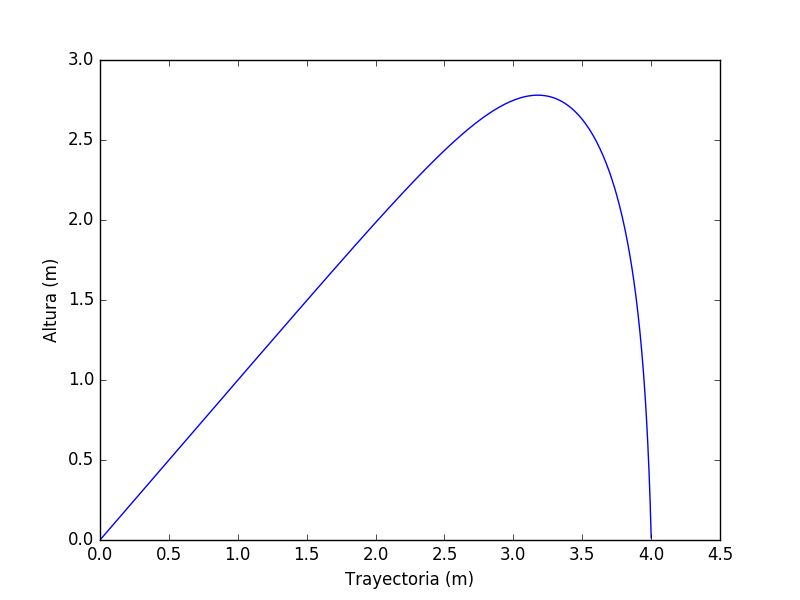
\includegraphics[width = \linewidth]{proyectil45.png}
    \caption{Movimiento de un proyectil con un ángulo inicial de 45$^\circ$ y una velocidad de 300m/s }
    \label{fig:proyectil45}
\end{figure}
En la Figura \ref{fig:proyectil45} se puede observar como varia la trayectoria en el eje $x$ y $y$ de un proyectil con un ángulo inicial de 45$^\circ$ y una velocidad de 300m/s. Después de que el proyectil alcanza su altura máxima, empieza a disminuir su velocidad en la dirección $x$, por lo que no alcanza a tener la trayectoria parabólica que se observaría si no se tuviera en cuenta la fricción del aire.

\begin{figure}[H]
    \centering
    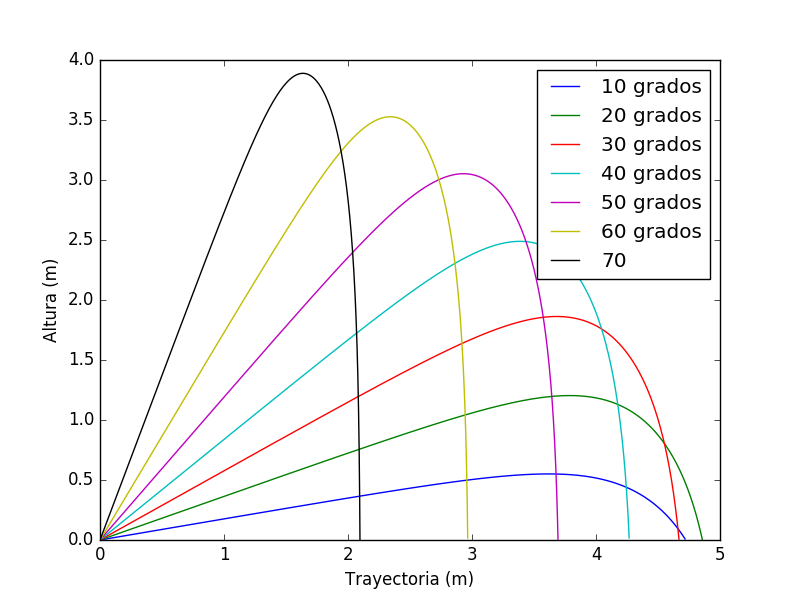
\includegraphics[width = \linewidth]{proyectilangulos.png}
    \caption{Movimiento de un proyectil con distintos ángulos iniciales}
    \label{fig:protectilangulos}
\end{figure}
En la Figura \ref{fig:protectilangulos} se puede observar como varia la trayectoria en el eje $x$ y $y$ de un proyectil con distintos ángulos iniciales. El ángulo que recorre la mayor distancia es el de 20$^\circ$ mientras que el que recorre la menor distancia es el de 70$^\circ$. Si no existiera la fricción del aire, el proyectil que recorreria la mayor distancia seria el de 45$^\circ$, mientras que los proyectiles lanzados con los ángulos (40$^\circ$-50$^\circ$) (30$^\circ$-60$^\circ$) (20$^\circ$-70$^\circ$) serían las mismas.

\section{Ecuaciones Diferenciales Parciales: Ecuación de difusión en una placa de Calcita}
\subsection{Condiciones de frontera fijas}

\begin{figure}[H]
    \centering
    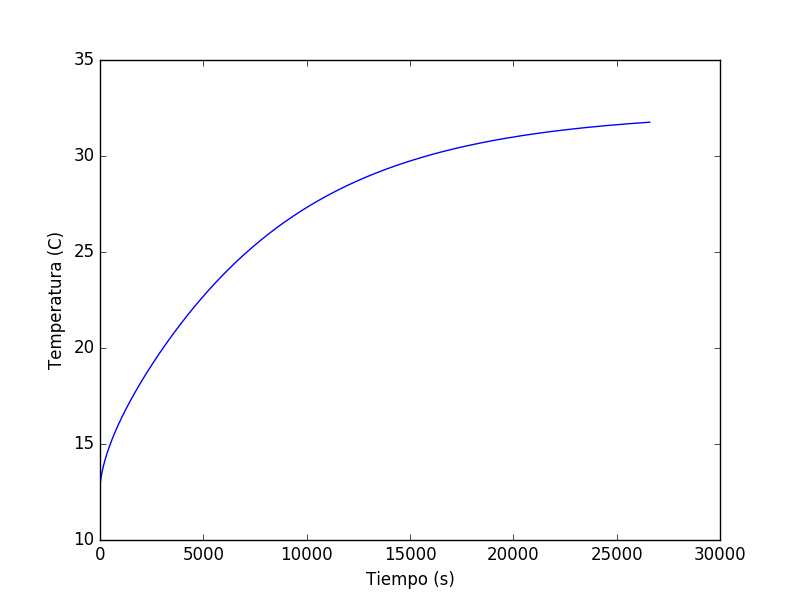
\includegraphics[width=\linewidth]{promediofija.png}
    \caption{Variación del promedio de la temperatura de la placa, cuando se tienen condiciones de frontera fijas}
    \label{fig:promediofija}
\end{figure}

En la Figura \ref{fig:promediofija} se puede observar que la placa llega a un estado de equilibrio cuando alcanza aproximadamente 32.5$^\circ$C.\\

\begin{figure}[H]
    \centering
    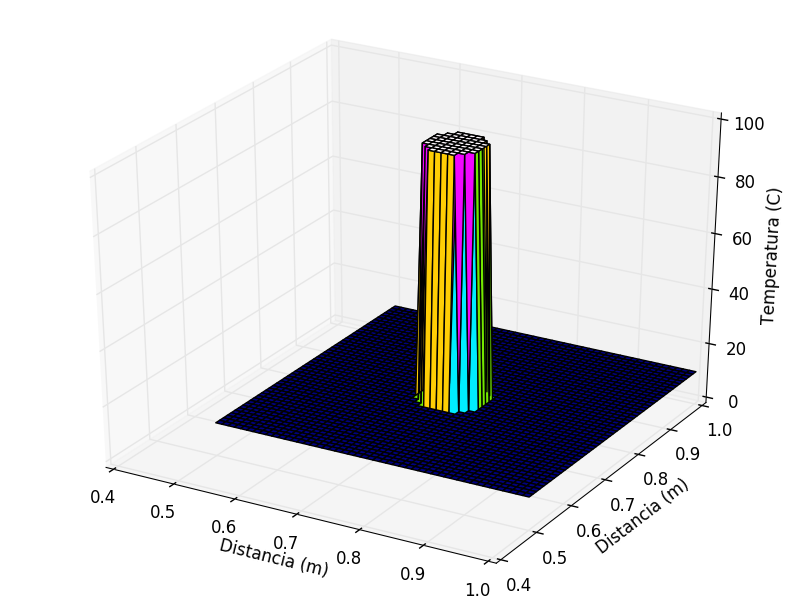
\includegraphics[width=\linewidth]{placafijainicial.png}
    \caption{Condición inicial de la placa de Calcita cuando se tienen condiciones de frontera fijas}
    \label{fig:placafijainicial}
\end{figure}

\begin{figure}[H]
    \centering
    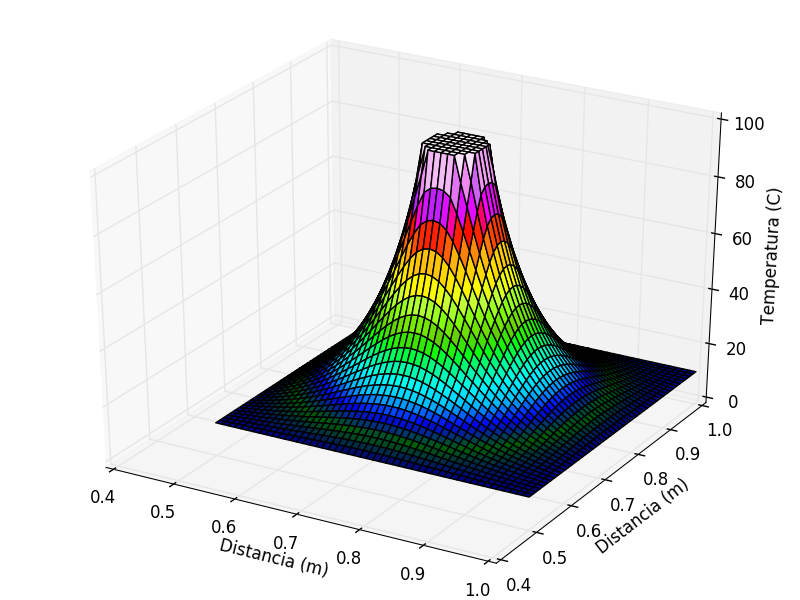
\includegraphics[width=\linewidth]{placafijaintermedio1.png}
    \caption{Condición intermedia de la placa de Calcita cuando se tienen condiciones de frontera fijas}
    \label{fig:placafijaintermedio1}
\end{figure}

\begin{figure}[H]
    \centering
    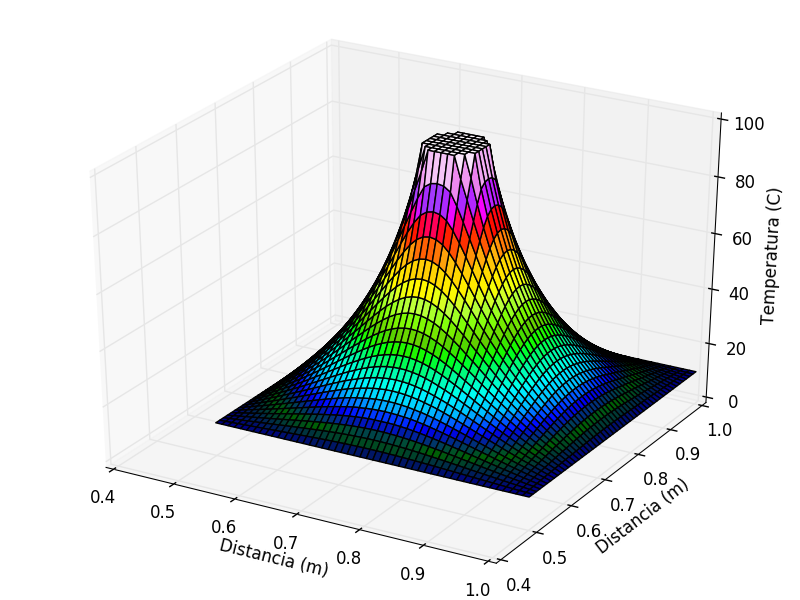
\includegraphics[width=\linewidth]{placafijaintermedio2.png}
    \caption{Condición intermedia de la placa de Calcita cuando se tienen condiciones de frontera fijas}
    \label{fig:placafijaintermedio2}
\end{figure}

\begin{figure}[H]
    \centering
    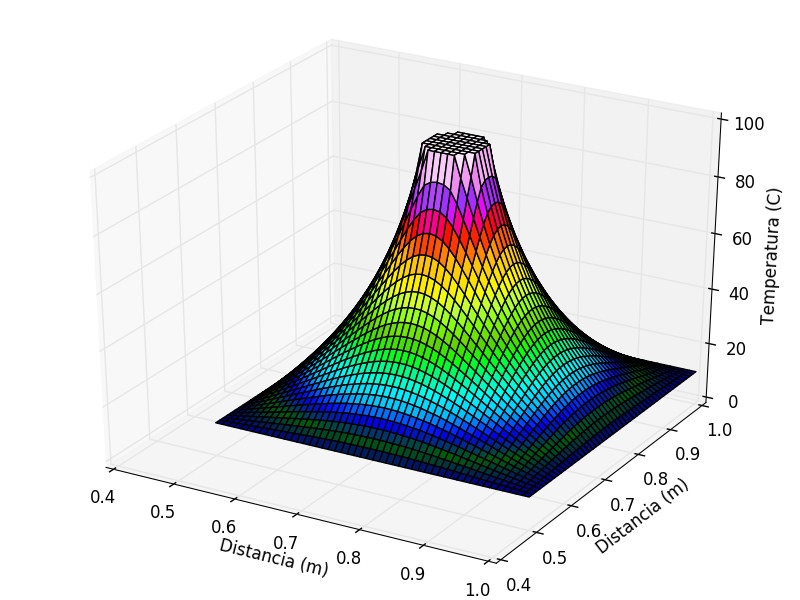
\includegraphics[width=\linewidth]{placafijafinal.png}
    \caption{Condición final de la placa de Calcita cuando se tienen condiciones de frontera fijas}
    \label{fig:placafijafinal}
\end{figure}

En las Figuras \ref{fig:placafijainicial}-\ref{fig:placafijafinal} se puede observar los distintos estados por los que pasa la placa hasta llegar al estado de equilibrio.\\
El estado de equilibrio en este caso se da debido a que las condiciones de frontera siempre se mantienen en la misma temperatura. Por eso mismo, es posible esperar que, si bien la temperatura de la placa aumenta con el tiempo, esta nunca va a llegar a los 100$^\circ$C.

\subsection{Condiciones de frontera libres}

\begin{figure}[H]
    \centering
    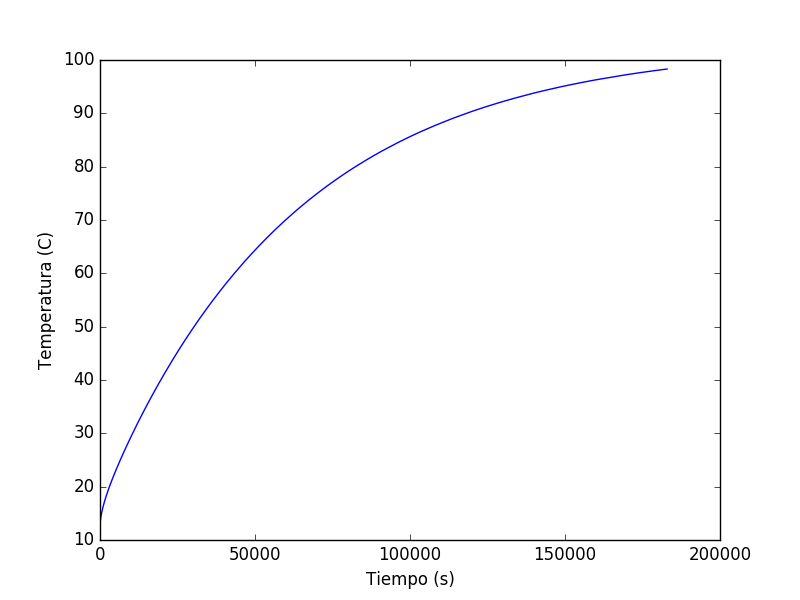
\includegraphics[width=\linewidth]{promediolibre.png}
    \caption{Variación del promedio de la temperatura de la placa, cuando se tienen condiciones de frontera libres}
    \label{fig:promediolibre}
\end{figure}

En la Figura \ref{fig:promediolibre} se puede observar que la placa llega a un estado de equilibrio cuando alcanza aproximadamente 100$^\circ$C.\\
\begin{figure}[H]
    \centering
    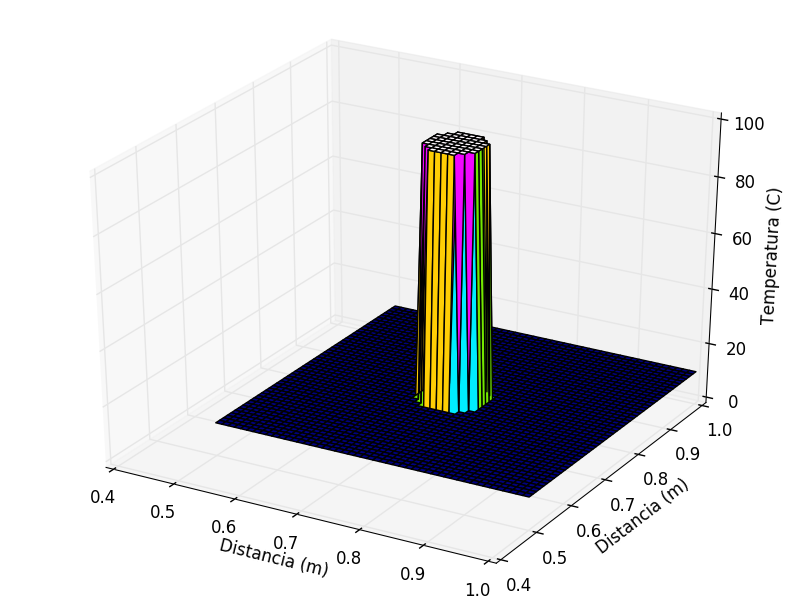
\includegraphics[width=\linewidth]{placalibreinicial.png}
    \caption{Condición inicial de la placa de Calcita cuando se tienen condiciones de frontera libres}
    \label{fig:placalibreinicial}
\end{figure}

\begin{figure}[H]
    \centering
    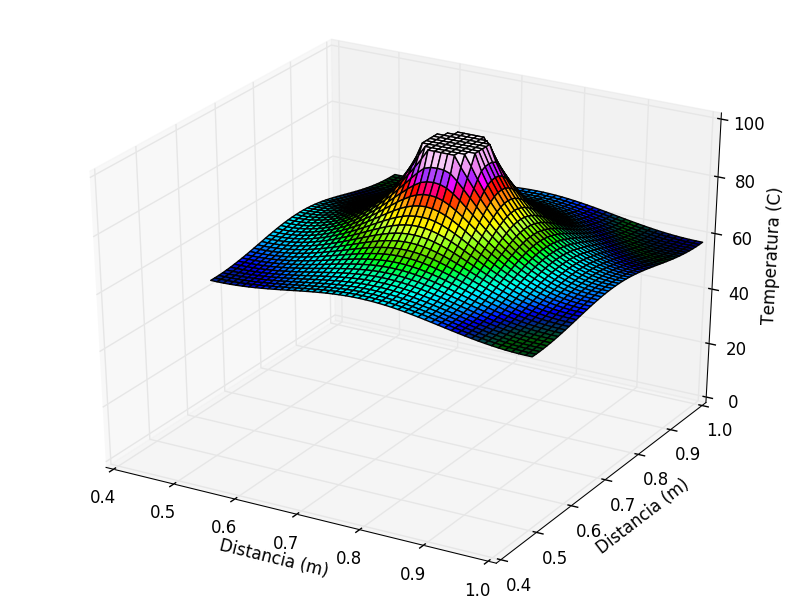
\includegraphics[width=\linewidth]{placalibreintermedio1.png}
    \caption{Condición intermedia de la placa de Calcita cuando se tienen condiciones de frontera libres}
    \label{fig:placalibreintermedio1}
\end{figure}

\begin{figure}[H]
    \centering
    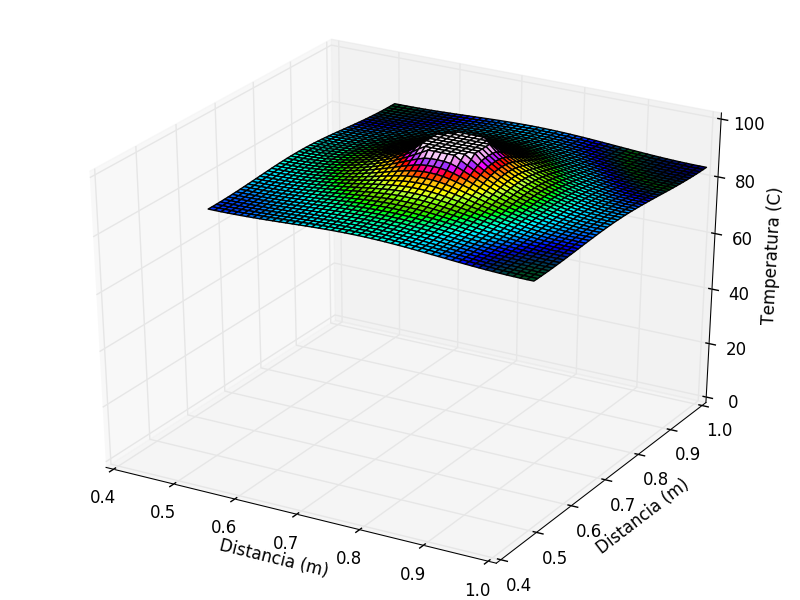
\includegraphics[width=\linewidth]{placalibreintermedio2.png}
    \caption{Condición intermedia de la placa de Calcita cuando se tienen condiciones de frontera libres}
    \label{fig:placalibreintermedio2}
\end{figure}

\begin{figure}[H]
    \centering
    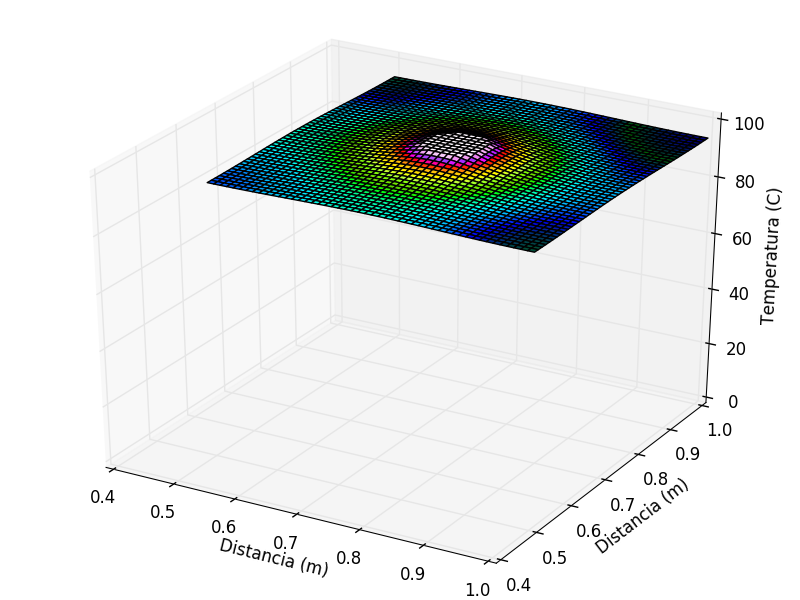
\includegraphics[width=\linewidth]{placalibrefinal.png}
    \caption{Condición final de la placa de Calcita cuando se tienen condiciones de frontera libres}
    \label{fig:placalibrefinal}
\end{figure}
En las Figuras \ref{fig:placalibreinicial}-\ref{fig:placalibrefinal} se puede observar los distintos estados por los que pasa la placa hasta llegar al estado de equilibrio.

\subsection{Condiciones de frontera periódicas}
\begin{figure}[H]
    \centering
    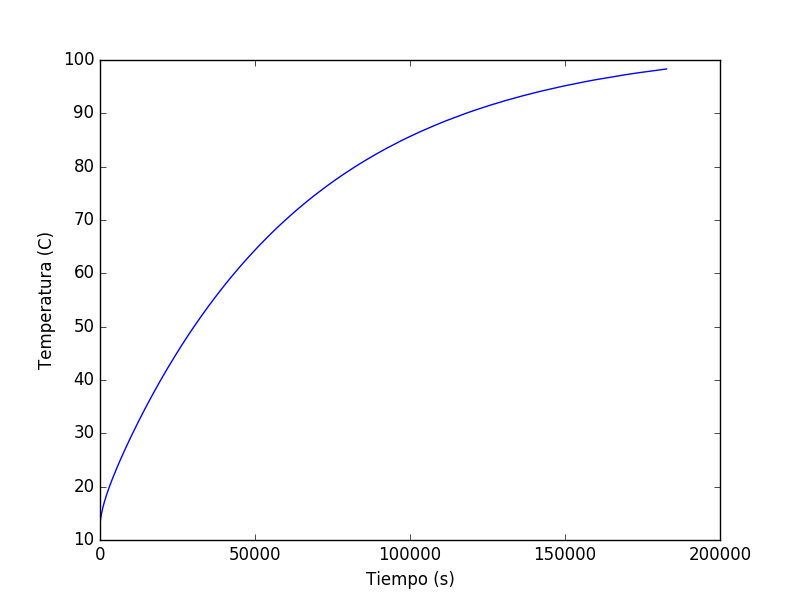
\includegraphics[width=\linewidth]{promedioperiodica.png}
    \caption{Variación del promedio de la temperatura de la placa, cuando se tienen condiciones de frontera periodicas}
    \label{fig:promediop}
\end{figure}
En la Figura \ref{fig:promediop} se puede observar que la placa llega a un estado de equilibrio cuando alcanza aproximadamente 100$^\circ$C.\\

\begin{figure}[H]
    \centering
    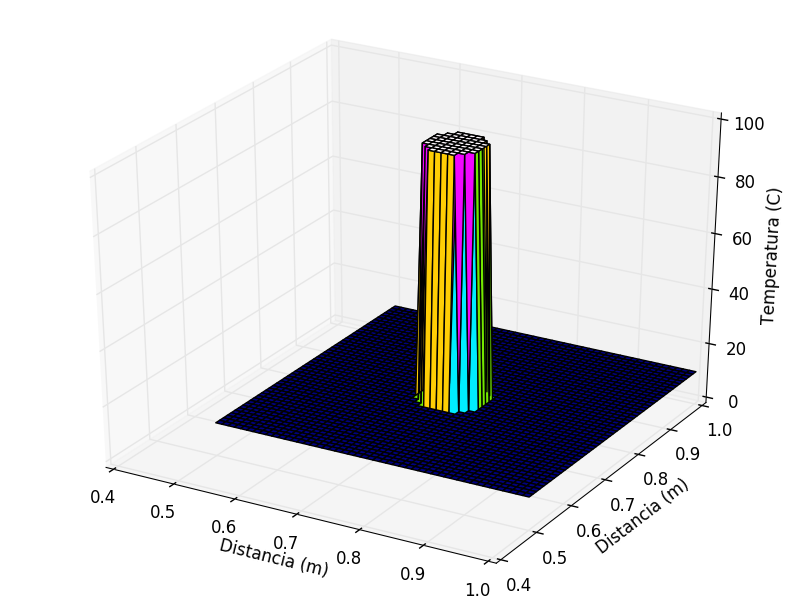
\includegraphics[width=\linewidth]{placaperiodicainicial.png}
    \caption{Condición inicial de la placa de Calcita cuando se tienen condiciones de frontera periodicas}
    \label{fig:placaperiodicainicial}
\end{figure}

\begin{figure}[H]
    \centering
    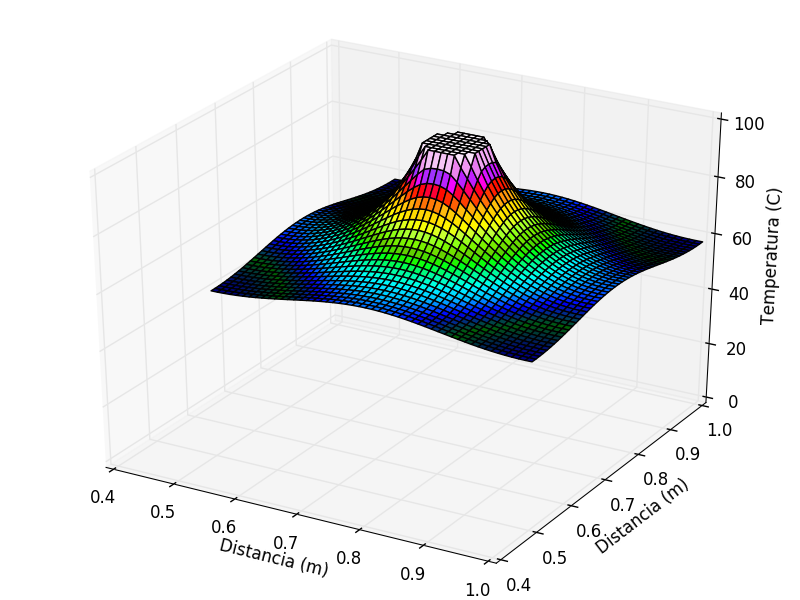
\includegraphics[width=\linewidth]{placaperiodicaintermedio1.png}
    \caption{Condición intermedia de la placa de Calcita cuando se tienen condiciones de frontera periodicas}
    \label{fig:placalibreintermedio1}
\end{figure}

\begin{figure}[H]
    \centering
    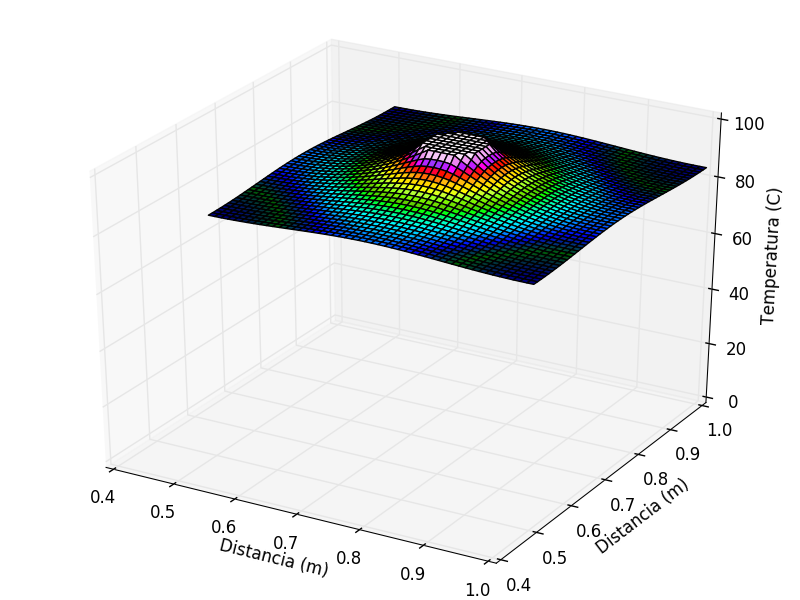
\includegraphics[width=\linewidth]{placaperiodicaintermedio2.png}
    \caption{Condición intermedia de la placa de Calcita cuando se tienen condiciones de frontera periodicas}
    \label{fig:placalibreintermedio2}
\end{figure}

\begin{figure}[H]
    \centering
    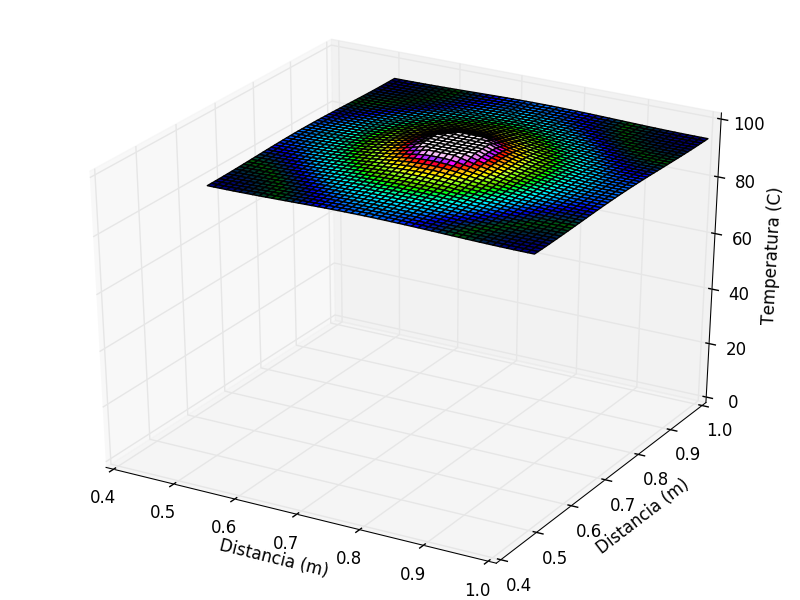
\includegraphics[width=\linewidth]{placaperiodicafinal.png}
    \caption{Condición final de la placa de Calcita cuando se tienen condiciones de frontera periodicas}
    \label{fig:placaperiodicafinal}
\end{figure}

En las Figuras \ref{fig:placaperiodicainicial}-\ref{fig:placaperiodicafinal} se puede observar los distintos estados por los que pasa la placa hasta llegar al estado de equilibrio.
\end{document}

